\subsection{Exclusive \WW}
\label{sec:exclWWCR}
\par While the 1 to 4-track region introduced in Table~\ref{tab:incWWCR} was 
rich in inclusive \WW\ events, replacing the 1 to 4-track selection criterion with the 
nominal \DZ\ selection criterion suppressed the inclusive \WW\ events and enhanced 
the exclusive \WW\ events. This is the exclusive \WW\ validation region. 

\par Although this region was discussed in Section~\ref{sec:incWW}, validation kinematic 
distributions are presented in this section. Figure~\ref{fig:exclWWCR} shows such 
distributions. The inclusive \WW contribution was scaled by 0.79 as discussed in Section~\ref{sec:incWW}. 
The exclusive \WW\ and $\tau\tau$ estimates were scaled by \fgam. Contributions from 
$VV$ were very small. Any other background processes were insignificantly small in comparison to 
the inclusive \WW\ contribution. 
  
\begin{figure}[!h]
\begin{subfigure}{0.5\textwidth}
   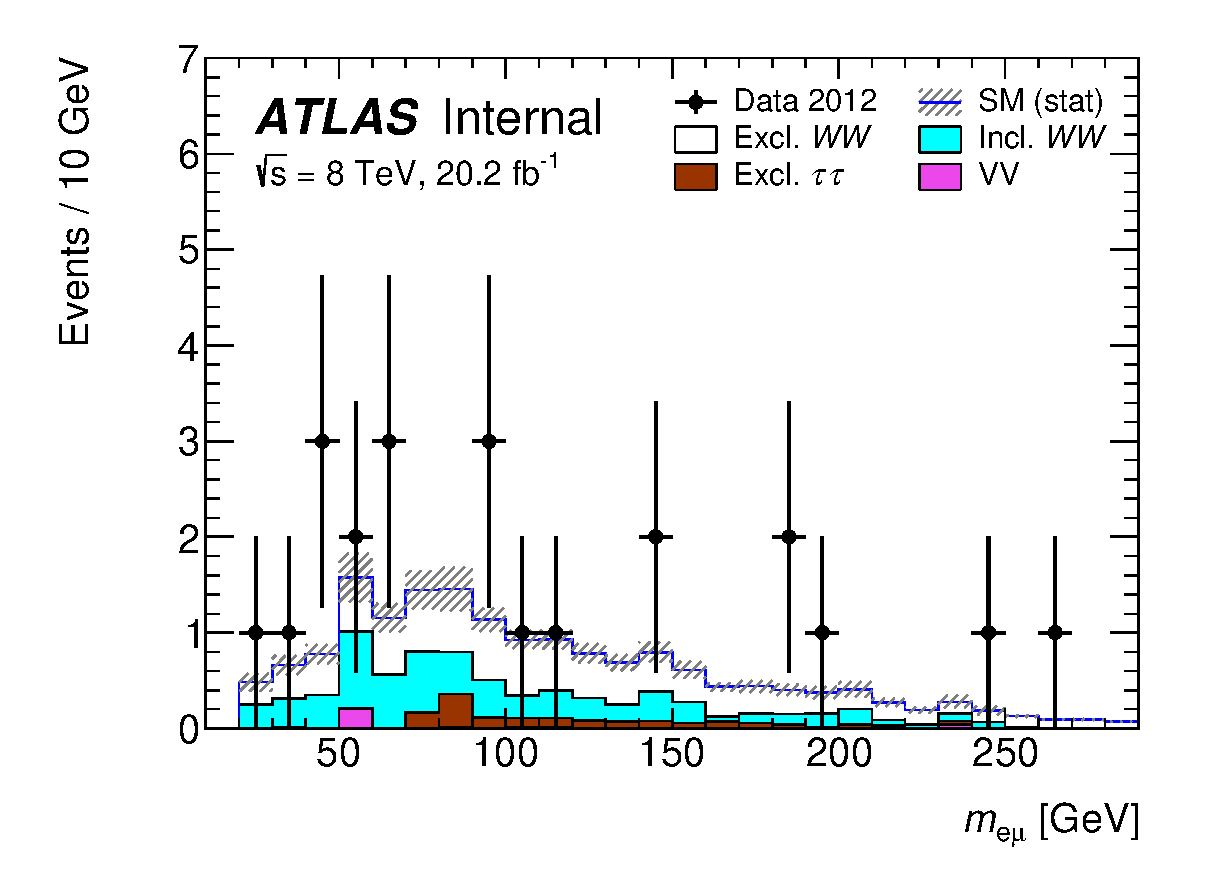
\includegraphics[width=\textwidth]{figures/emme-CutExcl1mm-Mll-lin.eps}
\end{subfigure}
\begin{subfigure}{0.5\textwidth}
   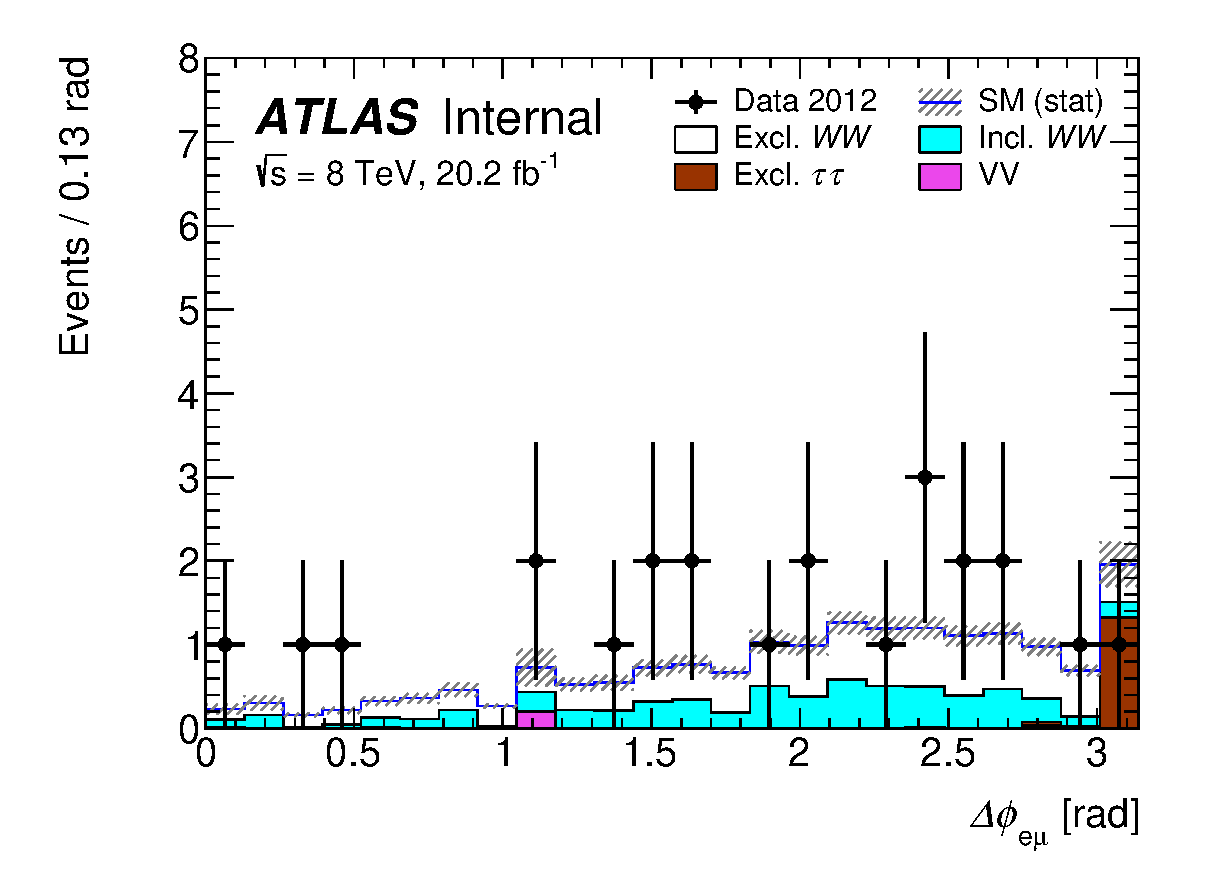
\includegraphics[width=\textwidth]{figures/emme-CutExcl1mm-DPhill-lin.eps}
\end{subfigure} 
\begin{subfigure}{0.5\textwidth}
   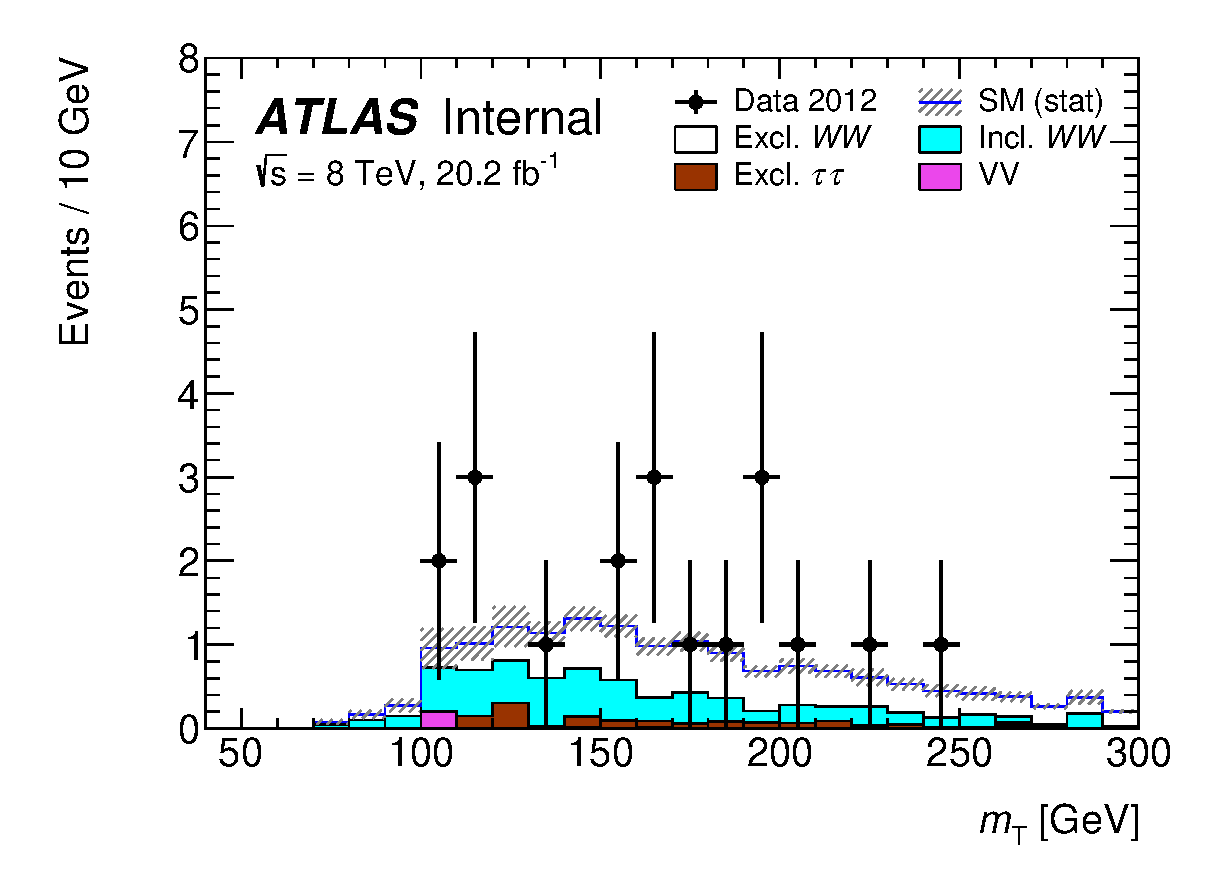
\includegraphics[width=\textwidth]{figures/emme-CutExcl1mm-MT-lin.eps}
\end{subfigure} 
\begin{subfigure}{0.5\textwidth}
   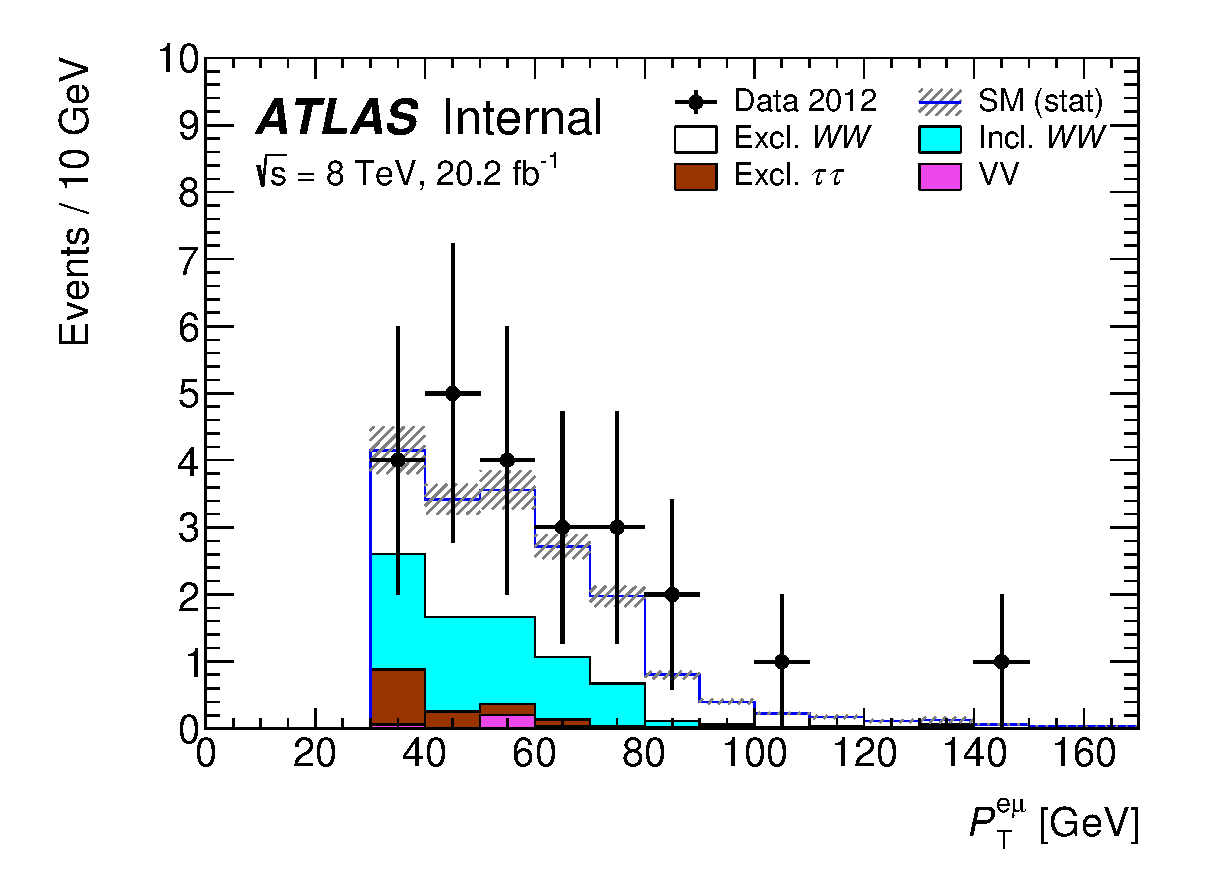
\includegraphics[width=\textwidth]{figures/emme-CutExcl1mm-Ptll-lin.eps}
\end{subfigure} 
\caption{Plots showing \memu, \dFem, \mT\ and \pTemu\ distributions in the exclusive \WW\ validation region}
\label{fig:exclWWCR}
\end{figure}

\par Overall Figure~\ref{fig:exclWWCR} shows reasonable agreement between data and 
predictions. A slight underestimation of exclusive \WW\ was observed across all the 
distributions. From counting the yields from all the processes and comparing them 
with the observed data, a normalization factor of 1.57$\pm$0.62 was extracted, to 
be additionally applied to the exclusive \WW\ contributions in the signal region. 
The uncertainty in this normalization factor resulted from propagation of 
uncertainties of each of the numbers that went into the calculation. 

\subsection{Inclusive \Ztau}
\label{subsec:ztau}
\par A \Ztau+jets-rich region was defined in data  
to validate background modelling in an environment dominated by inclusive processes. 
Table~\ref{tab:ZtauCR} summarizes the definition of this region.
Figure~\ref{fig:ZtauCR} shows some kinematic distributions in this validation 
region, after all the selection criteria summarized in Table~\ref{tab:ZtauCR} were applied.
The general slight disagreement between data and simulation was  
attributed to the mismodelling of the transverse momentum of the \Zboson, $p_T^Z$.
This mismodelling is well documented in Ref~\cite{Chelstowska:1636127}. While considerable efforts 
are normally applied to reweight the \Zboson\ \pt, \Ztau\ events were not 
a primary background in this analysis so such reweighting was observed to have insignificant effects on results. 

\begin{table}[!h]
\centering
\begin{tabular}{|l|r|}
\hline
& 	Selection 															\\
\hline\hline
 \multirow{3}{*}{Preselection }									&		Lepton $p_{\mathrm{T}}$ 25, 15 GeV	 		\\
																					&		OS and different flavour leptons 												 			\\
																					&		$m_{\ell\ell} > 10$ GeV 								\\
\hline
 \multirow{2}{*}{\Ztau}								&		$p_{\mathrm{T}}^{\ell\ell}<$30 GeV 				\\
									& 	$m_{\ell\ell}<80$ GeV 							\\
\hline
 \multirow{2}{*}{Exclusivity}	 					&		$|z_0^1-z_0^2|<1.0$ mm 							\\
											& 	$\Delta z_0 > 1.0$ mm 				\\	
\hline
\end{tabular}
\caption{\Ztau\ validation region definition.}
\label{tab:ZtauCR}
\end{table}

\begin{figure}[!h]
\begin{subfigure}{0.5\textwidth}
   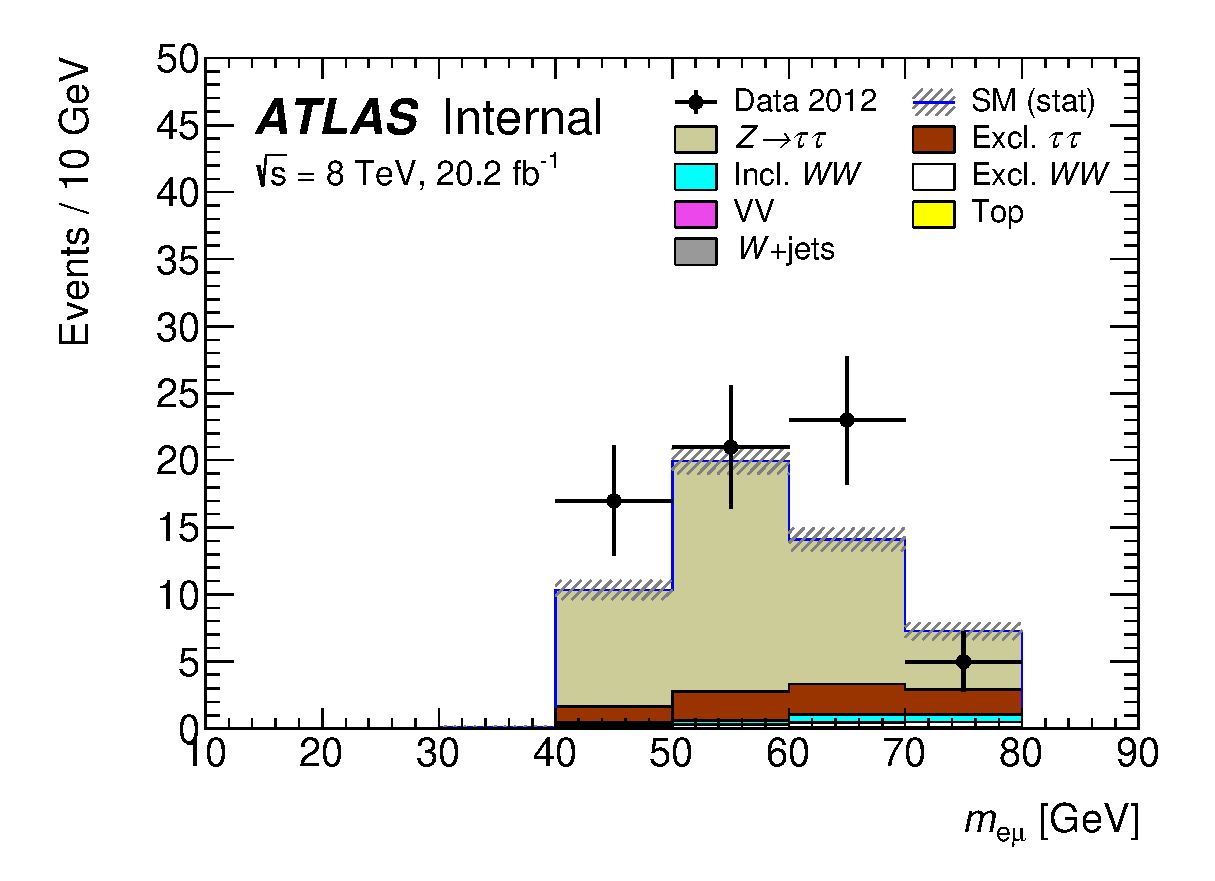
\includegraphics[width=\textwidth]{figures/emme-CutTopoMll-Mll_ztau-lin.eps}
\end{subfigure}
\begin{subfigure}{0.5\textwidth}
   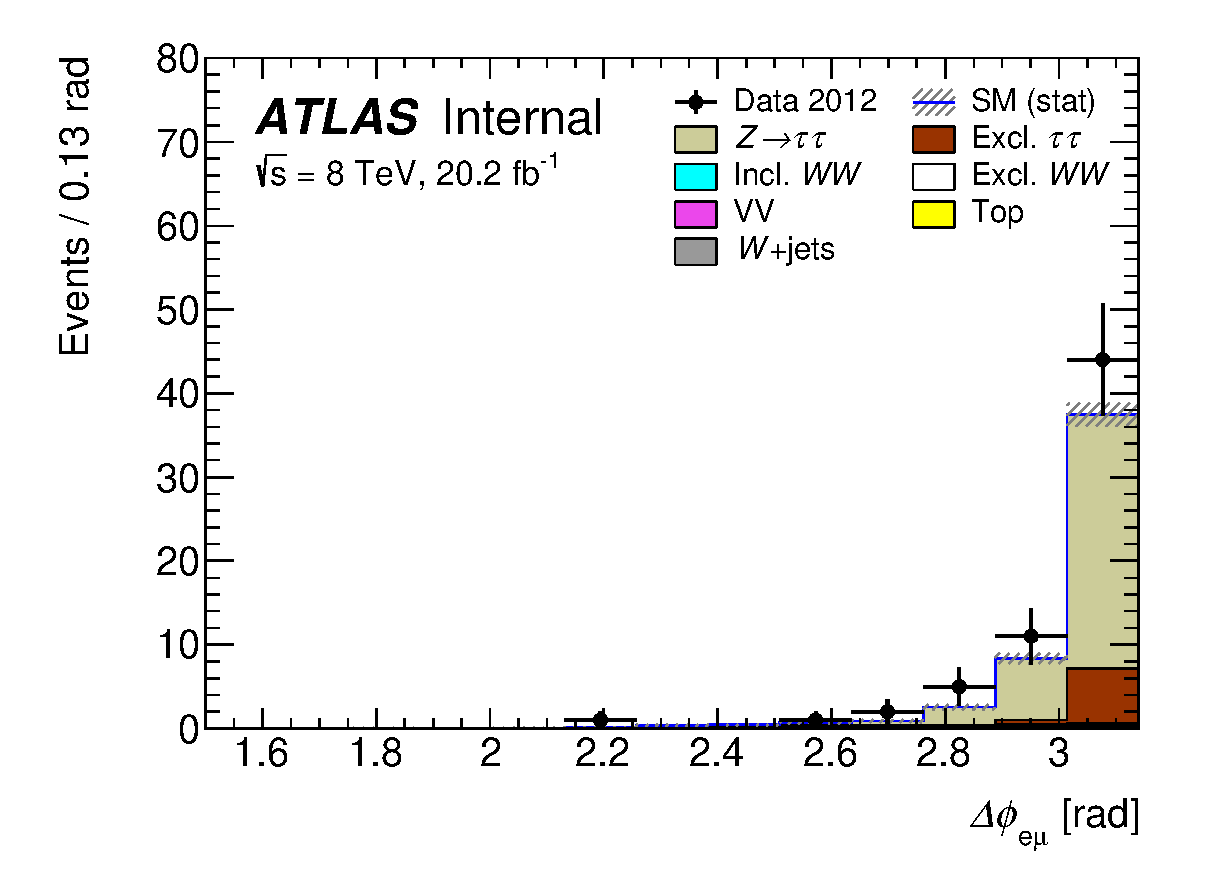
\includegraphics[width=\textwidth]{figures/emme-CutTopoMll-DPhill_ztau-lin.eps}
\end{subfigure} 
\begin{subfigure}{0.5\textwidth}
   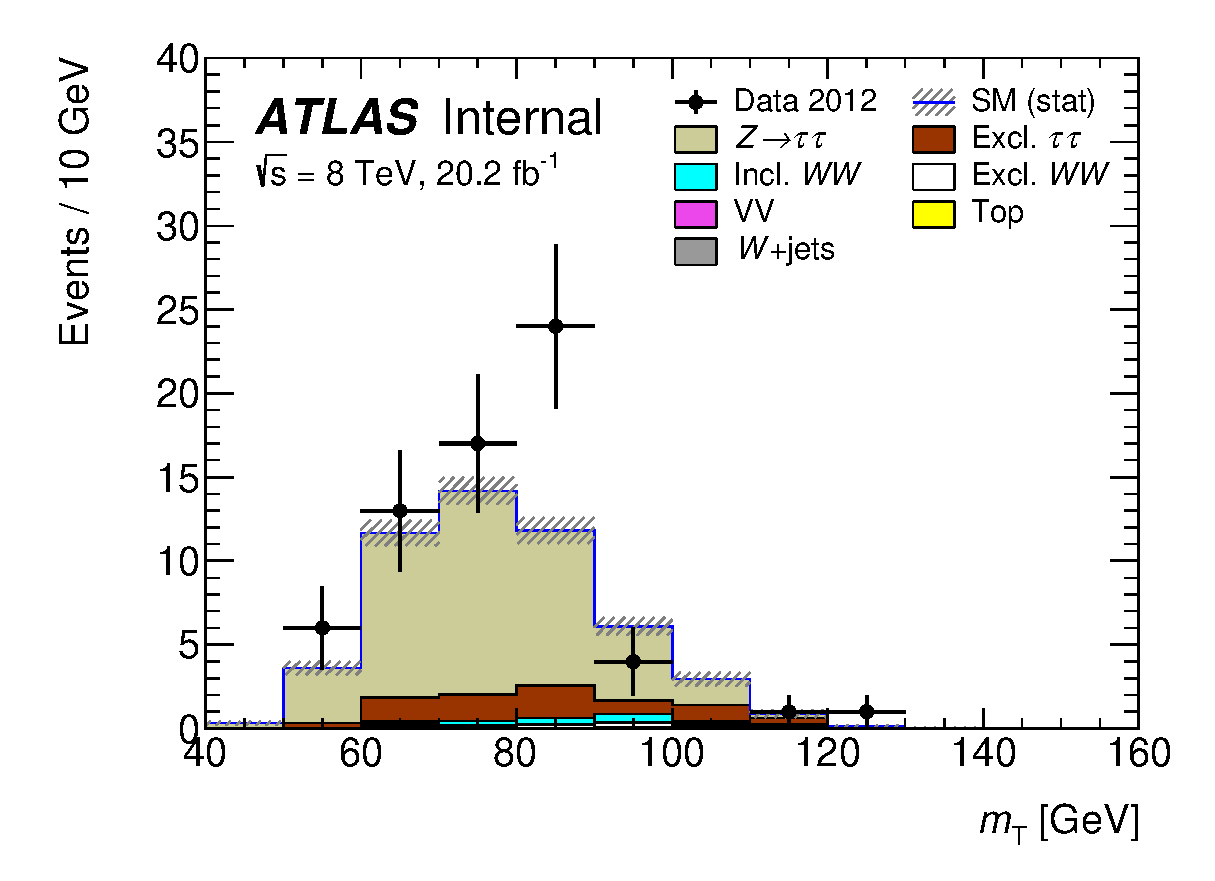
\includegraphics[width=\textwidth]{figures/emme-CutTopoMll-MT_ztau-lin.eps}
\end{subfigure} 
\begin{subfigure}{0.5\textwidth}
   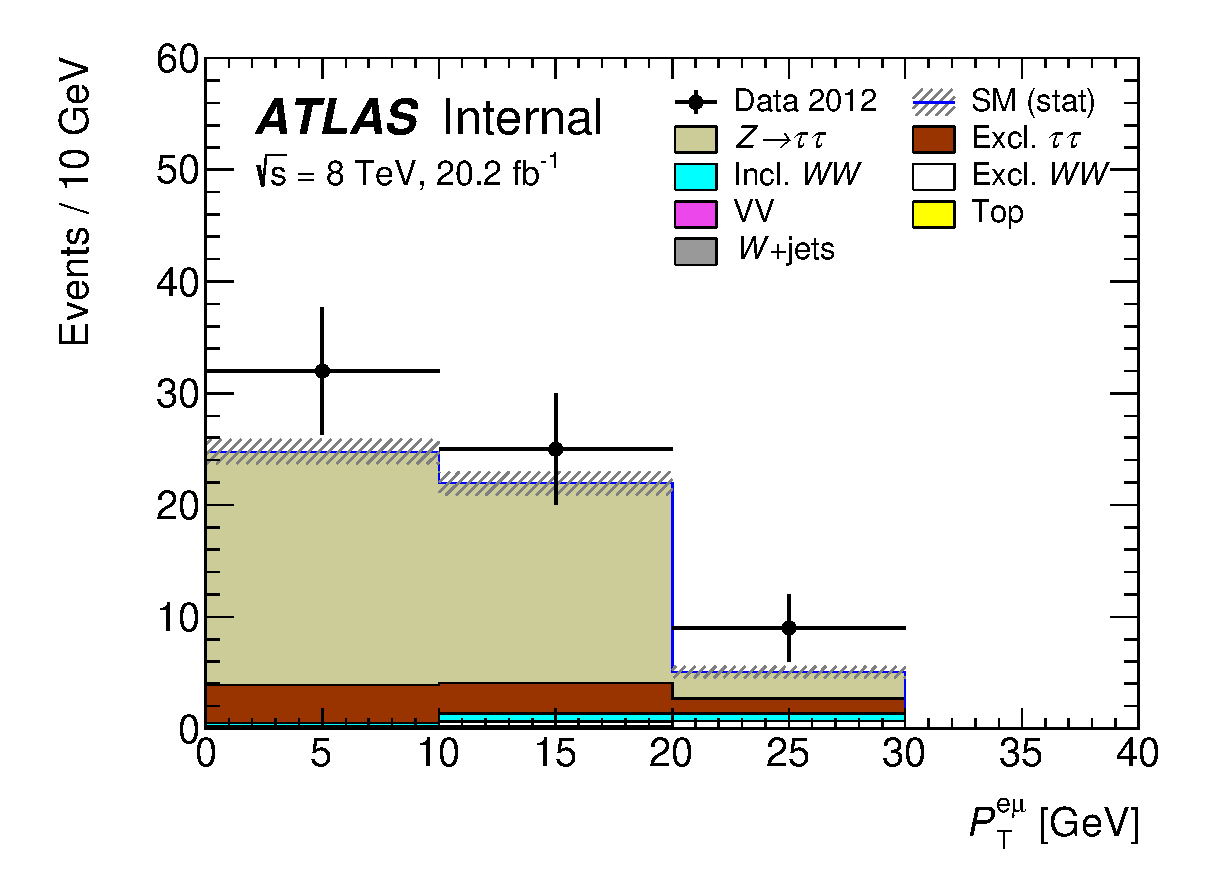
\includegraphics[width=\textwidth]{figures/emme-CutTopoMll-Ptll_ztau-lin.eps}
\end{subfigure} 
\caption{Plots showing \memu, \dFem, \mT\ and \pTemu\ distributions in the \Ztau\ validation region}
\label{fig:ZtauCR}
\end{figure}
